\documentclass[../main.tex]{subfiles}

\begin{document}
	\section{Risposte al gradino di sistemi di ordine 1 e 2}
		\begin{itemize}
			\item
				studiamo questa categoria perch\'e sono approssimazioni diffuse di sistemi reali.
			\item
				spesso cercheremo di ricondurci (attraverso controlli) a sistemi di questo tipo, perch\'e li sappiamo rappresentare molto bene e interpretare facilmente.
		\end{itemize}
		Studiamo solo la risposta forzata, perch\'e se questa diverge, allora anche la risposta libera diverger\'a. (se non \'e stabile BIBO, allora non \'e neppure stabile nella $ y_l $).
		
	\section{Sistemi di ordine 1}	
		La funzione di trasferimento di un sistema del 1° ordine strettamente proprio \'e:
		\[
			T(s) = \frac{b_0}{s+a_0}
		\]
		
		Se il sistema fosse semplicemente proprio, possiamo ricondurci al caso strettamente proprio.
		
		Dividiamo numeratore con denominatore:
		\[
			\tilde T(s) = \frac{\tilde a_1s + \tilde b_0}{s+\tilde a_0} = \tilde b_1 + \frac{\tilde b_0 - \tilde b_1 \tilde a_0}{s+\tilde a_0}
		\]
		\[
			Y_f(s) = \underbrace{\tilde b_1 U(s)}_{\begin{subarray} ccopia\ amplificata\\ dell'ingresso \end{subarray}} + \tilde T'(s)U(s)
		\]
		Troviamo la funzione resto $ \tilde T'(s) $ che \'e strettamente propria. Quindi possiamo concentrarci solo sul caso di sistema strettamente proprio. 
		
		La radice del denominatore \'e $ s_1 = -a_0 $:
		\begin{itemize}
			\item 
				$ a_0 \leq 0 \qquad \Rightarrow \qquad $ instabile BIBO.\\
				In particolare se $ a_0 < 0 $, la risposta forzata avr\'a andamento esponenziale nel tempo. Se $ a_0 = 0 $, la risposta forzata evolve come una retta.\\
				In entrambi i casi diverge.
			\item 
				$ a_0 > 0 \qquad \Rightarrow \qquad $ stabile BIBO.
		\end{itemize} 
	
		Concentriamoci solo sul caso della risposta stabile.
		\[
			T(s) = \frac{b_0}{s+a_0} = \frac{\frac{b_0}{a_0}}{1+\frac{1}{a_0}s} = \frac{k}{1+s \tau}
			\qquad 
			\begin{array}{l}
				k = \frac{b_0}{a_0} \quad \text{guadagno statico}
				\\[0.5cm]
				\tau = \frac{1}{a_0} \quad \text{costante di tempo}
			\end{array}
		\]
		
	\subsection{Risposta al gradino}
		Supponiamo che l'ingresso sia un gradino $ u(t) = \gr $. Calcoliamo la $ y_f(t) $:
		\begin{align*}
			y_f(t) &= \aLbrace{Y_f(s)} = \aLbrace{\frac{1}{s} \frac{b_0}{s+a_0}}
			\qquad
			Y_f(s) = \frac{b_0}{s(s+a_0)} = A\frac{1}{s} + B\frac{1}{s+a_0} 
			\\
			&A = \lim_{s \to 0} s \frac{b_0}{s(s+a_0)} = \frac{b_0}{a_0} = k
			\\
			&B = \lim_{s \to -a_0} (s+a_0)\frac{b_0}{s(s+a_0)} = -\frac{b_0}{a_0} = -k
			\\
			\Rightarrow\quad y_f(t) &= k (1-e^{t a_0}) = k(1-e^{-\frac{t}{\tau}}) \cdot \gr
		\end{align*}
		Studiamo la risposta forzata:
		\begin{itemize}
			\item 
				valore iniziale:
				\[
					\lim_{t \to 0^+} y_f(t) = 0 \quad \Rightarrow \quad y_f(0^+) = 0
				\]
			\item 
				valore iniziale della derivata, usiamo il teorema del valore iniziale:
				\[
					\dot y_f(0^+) = \lim_{s \to +\infty} s \cdot \aLbrace{\dot y_f(t)} = \lim_{s \to +\infty} \frac{s b_0}{s+a_0} = b_0 = \frac{k}{\tau}
				\]
				oppure
				\[ 
					\dot y_f(0^+) = \lim_{t \to 0^+} \frac{k}{\tau} e^{-\frac{t}{tau}} = \frac{k}{\tau} 
				\]
				$ \tau $ pu\'o essere interpretata come il tempo che impiegherebbe $ y_f(t) $ ad arrivare al suo valore di regime se continuasse con pendenza come in $ t = 0^+ $.
			\item 
				valore di regime, con il teorema del valore finale:
				\[
					y_f(\infty) = \lim_{t \to \infty} y_f(t) = \lim_{s \to 0} s Y_f(s) = \lim_{s \to 0} \frac{b_0}{s+a_0} = \frac{b_0}{a_0} = k
				\]
				oppure
				\[ 
					y_f(\infty) = \lim_{t \to \infty} k(1-e^{-\frac{t}{\tau}}) \cdot \gr = k 
				\]
		\end{itemize}
		
		\begin{figure}[H]
			\centering
			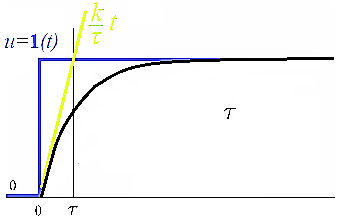
\includegraphics[width=0.4\textwidth]{risposta_gradino_ordine_1_2/sistema_ord_1}
			\caption{Grafico della risposta al gradino di un sistema di ordine 1.}
		\end{figure} 
		
	\subsubsection{Tempo di assestamento}
		Definiamo intanto:
		\[
			T_a = inf \left\lbrace \bar t : | y_f(t) - y_f(\infty) | \leq 0.05 \cdot y_f(\infty) \quad \forall t > \bar t \right\rbrace
		\]
		In questa categoria di sistemi si pu\'o verificare facilmente che: $ T_a \cong 3\tau $.
		
		\begin{figure}[H]
			\centering
			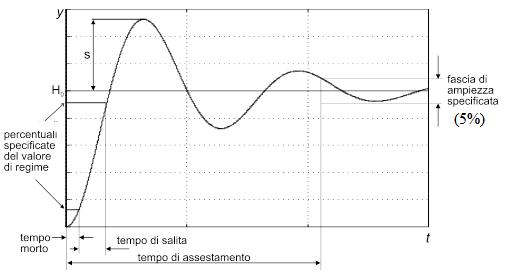
\includegraphics[width=0.6\textwidth]{risposta_gradino_ordine_1_2/sistema_ord_1_t_assest}
			\caption{Tempo di assestamento ed altri parametri.}
		\end{figure} 
		
	\section{Sistemi di ordine 2}
		\[ 
			T(s) = \frac{b_0}{s^2+a_1s+a_0}
		\]
		$ a_0 > 0 $ \'e condizione necessaria per avere:
		\begin{itemize}
			\item 
				stabilit\'a asintotica e BIBO. Infatti:
				\begin{itemize}
					\item 
						se $ a_0 = 0 $ avrei almeno una radice in zero.
					\item 
						se $ a_0 < 0 $ avrei sicuramente una variazione di segno (v. regola di Cartesio) e quindi una radice a $ \Re>0 $.
				\end{itemize}
			\item 
				poli complessi coniugati.
		\end{itemize}
		Riscriviamo la funzione di trasferimento raccogliendo $ a_0 $ a numeratore e a denominatore:
		\[ 
			T(s) = \frac{\frac{b_0}{a_0}}{1+\frac{a_1}{a_0}s+\frac{s^2}{a_0}} = \frac{k}{1 + 2\frac{\xi}{w_0}s + \frac{1}{w_0^2}s^2}
			\qquad
			\begin{cases}
				k = \frac{b_0}{a_0} \quad &\text{guadagno statico}
				\\
				w_0 = \sqrt{a_0} \quad &\text{pulsazione naturale}
				\\
				\xi = \frac{a_1}{2\sqrt{a_0}} \quad &\text{coefficiente di smorzamento}
			\end{cases}
		\]
		I poli di $T(s)$ sono:
		\[ 
			p_{1,2} = w_0(-\xi \pm \sqrt{\xi^2-1})
		\]
		Studiamo i poli per $ \xi \geq 0 $:
		\begin{itemize}
			\item 
				$ \xi = 0 \quad p_{1,2} =\pm w_0 \sqrt{-1} = \pm jw_0 \quad \text{radici puramente immaginarie}$
			\item 
				$ 0 < \xi < 1 \quad \text{due radici complesse coniugate con} \quad \Re = -w_0\xi \quad e \quad \Im = \pm w_0 \sqrt{1-\xi^2} $
				\[ 
					\left| p_{1,2} \right| = \sqrt{\Re^2 + \Im^2} = \sqrt{w_0^2\xi^2 + w_0^2(1-\xi^2)} = \sqrt{w_0^2} = w_0
				\]
				cio\'e le radici si trovano su una semi circonferenza (solo parte sinistra) centrata nell'origine e di raggio $ w_0 $.
			\item 
				$ \xi = 1 \quad p_{1,2} = -w_0 \quad molt=2 \quad \text{due radici reali coincidenti} $
			\item 
				$ \xi > 1 \quad \text{otteniamo due radici reali} $
		\end{itemize}
		Studiamo i poli per $ \xi < 0 $:
		\begin{itemize}
			\item troviamo una situazione simmetrica in cui le radici hanno tutte $ \Re > 0 $.
		\end{itemize}
		Quindi ricaviamo che $ \xi > 0 $ \'e \textbf{condizione necessaria e sufficiente} per la stabilit\'a BIBO.
		
	\subsection{Risposta al gradino}
		Analizziamo la risposta forzata del sistema al variare di $ \xi $:
	
	\subsubsection{$ \spadesuit \quad \xi < 0 $}
		La risposta forzata diverge.
		
	\subsubsection{$ \spadesuit \quad \xi = 0 $}
		\[
			Y_f(s) = \frac{kw_0^2}{s(s^2+w_0^2)} = \frac{A}{s} + B\frac{w_0}{s^2+w_0^2} + C\frac{s}{s^2+w_0^2}
			\qquad
			\begin{cases}
				A = k\\
				B = 0\\
				C = -k
			\end{cases}
		\]
		In uscita otteniamo una cosinusoide non smorzata:
		\[
			y_f(t) = k(1-\cos(w_0t)) \cdot \gr
		\]
		
	\subsubsection{$ \spadesuit \quad 0 < \xi < 1 $}
		\[ 
			y_f(t) = k \left[ 1 - \frac{e^{-w_0\xi t}}{\sqrt{1-\xi^2}} \sin\left( w_0 \sqrt{1-\xi^2} \cdot t + \arctan \frac{\sqrt{1-\xi^2}}{\xi} \right) \right] \cdot \gr 
		\]
		Applichiamo il teorema del valore iniziale:
		\[ 
			y_f(0^+) = \lim_{t \to 0^+} = \lim_{s \to \infty} s Y_f(s) = \lim_{s \to \infty} \frac{k}{1 + 2\frac{\xi}{w_0}s + \frac{1}{w_0^2}s^2} = 0
		\]
		\[ 
			\dot y_f(0^+) = \lim_{s \to \infty} s \left[ sY_f(s) - y_f(0^-) \right] = \lim_{s \to \infty} \frac{k\ s}{1 + 2\frac{\xi}{w_0}s + \frac{1}{w_0^2}s^2} = 0
		\]
		cio\'e parte con pendenza nulla dall'origine.
		
		Vediamo come dipende la risposta forzata dai coefficienti $ \xi $ e $ w_0 $:
		\begin{itemize}
			\item 
				$ w_0 $ fissato:\\
				se $ \xi $ \'e piccolo le oscillazioni si smorzano lentamente.
			\item 
				$ \xi $ fissato:\\
				se $ w_0 $ \'e grande, la frequenza aumenta e il grafico risulta pi\'u schiacciato verso l'asse y.
		\end{itemize}
		\begin{figure}[H]
			\centering
			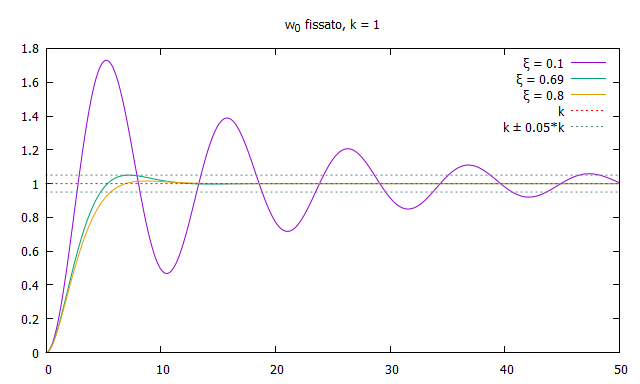
\includegraphics[width=0.8\textwidth]{risposta_gradino_ordine_1_2/sistema_ord_2_w_cost}
			\caption{Grafico della risposta forzata nel tempo al variare di $ \xi $, con $ w_0 $ fissato.}
		\end{figure} 
		\begin{figure}[H]
			\centering
			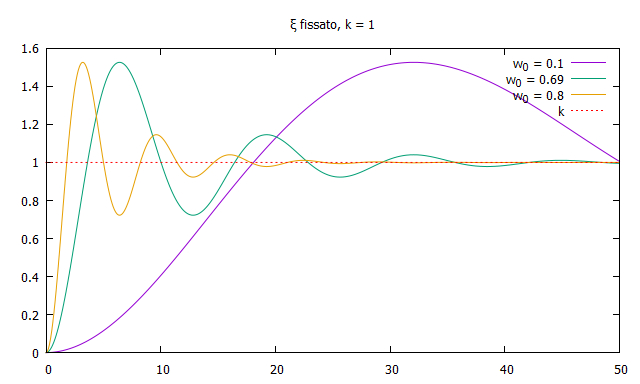
\includegraphics[width=0.8\textwidth]{risposta_gradino_ordine_1_2/sistema_ord_2_xi_cost}
			\caption{Grafico della risposta forzata nel tempo al variare di $ w_0 $, con $ \xi $ fissato.}
		\end{figure}
		
	\subsubsection{Parametri}
		\begin{itemize}
			\item 
				$ y_m - k $ sovra-elongazione massima.
			\item 
				$ S_m = \frac{y_m-k}{k} = e^{-\frac{\pi \xi}{\sqrt{1-\xi^2}}} $ sovra-elongazione massima relativa.\\
				Si pu\'o ricavare che se $ \xi > 0.69 $, la curva entra nel $ 5\% $ del valore di regime e non ne esce pi\'u.
			\item 
				$ T_r $ tempo di ritardo:\\ 
			tempo che impiega la curva ad arrivare al $ 10\% $ del valore di regime.
			\item 
				$ T_s $ tempo di salita:\\
			tempo che impiega la curva per passare dal $ 10\% $ al $ 90\% $ del valore di regime.
			\item 
				$ T_m = \frac{\pi}{w_0 \sqrt{1-\xi^2}} $ tempo di sovra-elongazione massima.
			\item 
				$ T_a $ tempo di assestamento.\\
				Se $ \xi \leq 0.69 $ allora $ T_a \cong \frac{3}{w_0 \xi} $.\\
				Se volessi un sistema di ordine 2 con $ T_a \leq \bar t $, dovrei imporre $ \underbrace{-w_0 \xi}_{ \re{p_{1,2}} } \leq -\frac{3}{\bar t} $.
		\end{itemize}
		\begin{figure}[H]
			\centering
			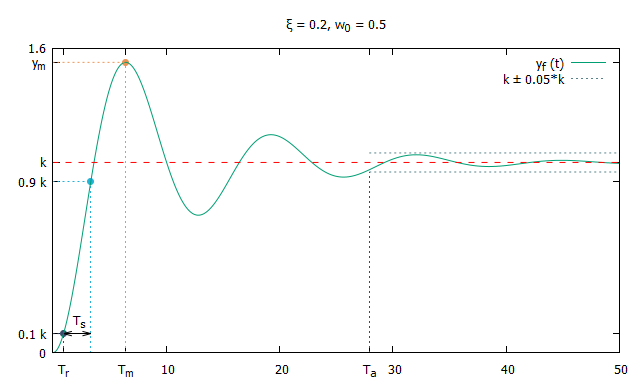
\includegraphics[width=0.8\textwidth]{risposta_gradino_ordine_1_2/parametri}
		\end{figure}
		
	\subsubsection{$ \spadesuit \quad \xi \geq 1 $}
		I poli sono entrambi reali e negativi:
		\[ 
			T(s) = \frac{k}{1 + 2\frac{\xi}{w_0}s  +\frac{1}{w_0^2}s^2} = \frac{k}{(1+s\tau_1)(1+s\tau_2)}
		\]
		\[ 
			p_1 = -\frac{1}{\tau_1} \qquad p_2 = -\frac{1}{\tau_2}
		\]
		\begin{itemize}
			\item 
				$ \xi = 1 \quad \Rightarrow \quad \tau_1 = \tau_2 $
				otteniamo 2 poli coincidenti: $ p = -\frac{1}{\tau} \quad m = 2 $
				\[ 
					Y_f(s) = A\frac{1}{s} + B\frac{1}{s+\frac{1}{\tau}} + C\frac{1}{(s+\frac{1}{\tau})^2} 
				\]
				\[ 
					y_f(t) = \left[ A + Be^{-\frac{t}{\tau}} + C t e^{-\frac{t}{\tau}} \right] \cdot \gr
				\]
			\item 
				$ \xi > 1 $
				\[ 
					Y_f(s) = A\frac{1}{s} + B\frac{1}{s+\frac{1}{\tau_1}} + C\frac{1}{s+\frac{1}{\tau_2}} 
				\]
				\[ 
					y_f(t) = \left[ A + Be^{-\frac{t}{\tau_1}} + Ce^{-\frac{t}{\tau_2}} \right] \cdot \gr 
				\]
				Nel complesso il sistema si comporta quasi come un sistema del 1° ordine.\\
				Osservazioni:
				\begin{itemize}
					\item 
						non esistono sovra elongazioni: la derivata \'e nulla solo nell'origine
					\item 
						$ T_a $ dipende fortemente dal polo pi\'u "lento" (quello con $ \tau $ pi\'u grande):
						\begin{align*}
							\frac{\tau_1}{\tau_2} << 1 \quad &\Rightarrow \quad T_a \cong 3 \tau_2
							\\
							\frac{\tau_1}{\tau_2} = 0.2 \quad &\Rightarrow \quad T_a \cong 3.22 \tau_2
							\\
							\frac{\tau_1}{\tau_2} = 0.5 \quad &\Rightarrow \quad T_a \cong 3.68 \tau_2
							\\
							\frac{\tau_1}{\tau_2}\ =\ 1 \quad &\Rightarrow \quad T_a \cong 4.75 \tau_2
						\end{align*}
						Spesso si usa il valore \textit{conservativo}: $ T_a < 5 \tau_2 $
				\end{itemize}
		\end{itemize}
\end{document}